\section{Discussion and Future Work}
\label{sec:discuss} In this section, we discuss the related issues
of our approach.

\textbf{Aligning client code of similar functionalities.} As shown
in Table~\ref{table:analyzingclient}, our approach sometimes fail to
align client code. For some considerations, programmers may
implement one functionality as one class or one method in one
version but implement the same functionality as multiple classes or
methods. One feasible way to align these functionalities is to
analyze them dynamically. For example, Jiang and
Su~\cite{jiang2009automatic} propose an approach to mine code
snippets of similar functionalities. We plan to introduce their
approach for those unmatched classes or methods in our future work.
%\begin{figure}[t]
%\centering
%\includegraphics[scale=1,clip]{figure/replaceableAPI.eps}\vspace*{-1.5ex}
% \caption{Mined API mapping}\vspace*{-3.5ex}
% \label{fig:minedapis}
%\end{figure}

\textbf{Mining richer API mapping.} As shown in
Table~\ref{table:compare}, although we use ten large projects as
subjects, our mined API mapping does not achieve high recalls. For a
given library, these projects still do not provide adequate source
files for mining. Our previous
work~\cite{thummalapenta07parseweb,thummalapentaase08spotweb} shows
that it is feasible to use the entire open source code on the web as
subjects for mining with the help of code search engines such as
Google code search\footnote{\url{http://www.google.com/codesearch}}.
We plan to leverage those search engines to mine richer API mapping
in our future work.

\textbf{Ranking mined mapping relations.} One API class or method
can be mapped to more than one class or method. For example, both
\CodeIn{java.lang.Boolean}$\leftrightarrow$ \CodeIn{System.Boolean}
and \CodeIn{java.lang. Boolean}$\leftrightarrow$
\CodeIn{System.Byte} are mined as mapping relations of API classes
in our experiment. When comparing with CSharp2Java, we choose the
formal to generate mapping files as the support of the former is 46
whereas the support of the latter is 4. However, in some cases, the
API mapping with the highest support is not necessarily the best
choice. For example, \CodeIn{java.util.ArrayList} is mapped to
\CodeIn{System.Collections.ArrayList} by support values. The Java
class support generic programming, whereas the C\# class does not.
Consequently, the Java class seems to be better mapped to
\CodeIn{System.Collections.Generic.List} as this C\# class supports
generic programming. We plan to develop some ranking techniques for
this issue in future work.


\begin{figure}[t]
\centering
\includegraphics[scale=1,clip]{figure/n2n.eps}\vspace*{-1.5ex}
 \caption{Merging technique}\vspace*{-3.5ex}
 \label{fig:n2n}
\end{figure}
\textbf{Mining more n-to-n mapping relations of API methods.} As
shown in Table~\ref{table:minedresults}, most mined mapping
relations of API methods describe one-to-one relations.
Algorithm~\ref{alg:mapATG} merges next APIs in a forward strategy.
For the example shown in Figure~\ref{fig:n2n}, if the algorithm
merges \CodeIn{method1()} and \CodeIn{method2()} but fails to find a
match, the algorithm tries to merge \CodeIn{method3()}. In some
cases, a match can be found if the algorithm merges
\CodeIn{method4()} instead of \CodeIn{method3()}. We plan to refine
the algorithm so that it can mine more n-to-n relations in future
work.

\textbf{Migrating n-to-n mapping relations of API methods.} A mined
n-to-n mapping of API methods may have multiple outputs and
complicated internal data processes. Our defined API transformation
graphs help find out all essential API methods. However the graph do
not describe adequate details to support automatic translations. For
example, we need to manually add an \emph{or} operator for the two
outputs of the API mapping shown in Figure~\ref{fig:example}. We pan
to add more details so that we can automate migrating of n-to-n
mapping relations in our future work.

\textbf{Migrating unmapped APIs.} Our approach mines API mapping of
methods that has mapped inputs, mapped outputs, and similar
functionalities. Consequently, mined API mapping can be migrated
automatically. However, some APIs between two languages cannot
satisfy all the three criteria. For these APIs, if outputs are
unmapped, our approach can simply ignores outputs when outputs are
not used in client code. If inputs or functionalities are unmapped,
we plan to develop techniques that analyze how two versions of a
project deal with the problem for some reusable code snippets in
future work.
